% !TEX root = ../my-thesis.tex
%
\chapter{AutoML with an Ensemble of Optimizers}
\label{sec:approach}
As outlined in the previous chapter, in theory any optimization approach under a resource budget is limited to a set of problem classes, where it can find a solution that is better than any solution another optimization approach could find for the same problem class, i.e. where the approach is superior.
For an actual use-case, as for instance AutoML, it would be necessary to either have significant domain knowledge or to had conducted a broad empirical evaluation to select the optimizer that have a high chance of performing superior for a newly encountered problem class.
This can be avoided, if during the optimization process a set of optimizers would be evaluated in the context of the presented optimization problem and the most apt one would be applied automatically.\newline
Furthermore, it was argued how a separation of the optimization space into model selection and model configuration spaces by optimization space transformations could be beneficial.
The anticipated advantages are a speed-up at first, because the dimensionality of the input space for an optimizer can be reduced.
Secondly, the best suited optimizer for the model configuration can be selected independently from the constructed pipeline after the model selection.\newline
Although this approach could be generalized to any form of algorithm selection and hyperparameter configuration problem, this thesis focusses on the AutoML use-case and therewith has to address well suited machine learning pipelines as an expected output for a wide variety of datasets as an input.
Thus, the constructed pipelines should be able to be as sophisticated as necessary to suit the complexity of any possible input dataset.
Therewith, the approach has the additional requirement of preventing overly stringent limitations of the pipeline topology such as a fix length or solely linear compositions.\newline
In the following chapter such a method will be presented and applied to the AutoML use-case.
This approach will be explained in the following steps in separate sections:
\begin{enumerate}
    \item A short overview how model selection and configuration spaces can be separated for this approach
    \item The structure of the model selection optimization space and how the optimization will be performed to enable the selection of different optimizers for model configuration out of an embedded optimizer ensemble
    \item The structure of the model configuration optimization space and which benefits can be utilized from using and re-using the different optimizers of the ensemble
\end{enumerate}

\section{Separation of Model Selection and Configuration}
\label{sec:approach:separation}
A usual AutoML optimization search space is a joint space for model selection and model configuration consisting out of a set of components, which can be used to construct a machine learning pipeline, and based on the selected components, a valid configuration has to be created.
Since in the joint optimization space the selected components are not known beforehand, the dimensionality of this space has to be selected for a fix parametrization size.
Hence, the model configuration can only create parameter configurations with a pre-defined size as a constraint and the set of pipeline components for model selection can only contain components whose configuration does not exceed this size.\newline
If the model selection and the model configuration steps are performed sequentially on separated optimization spaces, the dimensionality of the model configuration space can depend on the outcome of the model selection step and have the necessary dimensionality for the constructed pipelines parametrization.\newline
Similar to ReinBo and Mosaic, the model selection space is represented by a tree structure.
After the optimization method reaches a leaf node and has therewith complete and valid pipeline structure, the size of the required configuration becomes clear.
Any leaf node is for this reason the connection point and foundation for a model configuration space and the configuration requirements can be deduced.
Thus, dimensionality and structure of the optimization space for the model configuration can be determined from the configuration requirements of the pipeline represented in this leaf node.

\section{Model Selection with MCTS}
\label{sec:approach:selection}
While the overall goal of the model selection step is to construct a pipeline out of a set of pipeline components, in this approach two additional sub-goals come in addition as supplementary requirements:
\begin{enumerate}
    \item The constructed pipeline should be able to be constructed more flexible and more sophisticated than in ReinBo and Mosaic, i.e. have an unrestricted length and no constraints regarding linearity.
    \item The model selection step should be able to evaluate the different optimization methods and their performance regarding the input dataset or even regarding the model configuration for specific pipeline components in the context in the dataset.
    With such an approach, the the most suitable optimizer can be detected and exploited, which will be the key concept for creating an optimizer ensemble.
\end{enumerate}
In the following, both sub-goals will be addressed.
The next two sub-sections tackle the first sub-goal by modelling the model selection process as a graph search problem as first and describing this search graph in more detail afterwards.
Thereafter, in the third sub-section a formalization of the ensemble concept for multiple optimizers is given in the form of a Multi-Armed Bandit problem.
Finally, in the fourth sub-section it is illustrated how both sub-goals can be achieved during the model selection by performing a MCTS.

\subsection{Model Selection as a Graph Search Problem}
\label{sec:appraoch:selection:search}
A machine learning pipeline can vary heavily in structure and complexity.
For example, simple using a Decision tree as the only component as well as many components in a more sophisticated topology as in figure~\ref{fig:appraoch:complex-pipeline} are valid pipelines and depending on the concrete input dataset, both variants could be the optimal output of the model selection step.
\begin{figure}[ht!]
    \centering
    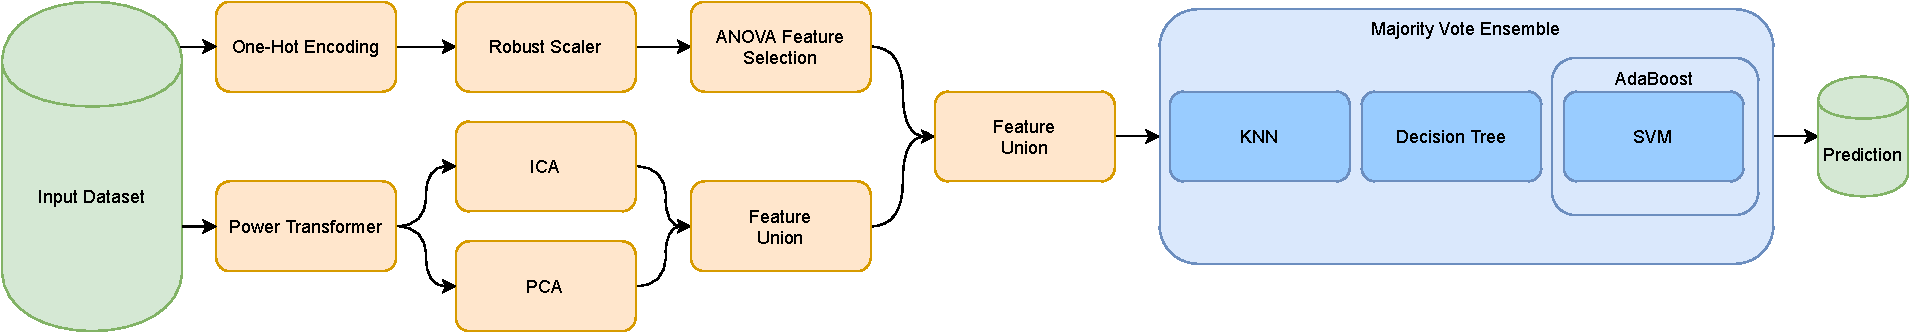
\includegraphics[width=\textwidth]{gfx/Figures/Approach/ComplexPipeline.pdf}
    \caption{An example of a complex machine learning pipeline with a higher length and a non-linear topology. Input dataset and output prediction data are shown in green, pre-processing components in orange and the machine learning components constructing the machine learning model in blue.}
    \label{fig:appraoch:complex-pipeline}
\end{figure}
Since ReinBo and Mosaic solve their model selection tasks by defining a fix pipeline length and creating a model selection tree containing every combinatorial possible combination from a few different component types, these approaches do not allow complex pipelines.\newline
Other approaches, as for example ML-Plan, TPOT or RECIPE utilize hierarchical task network planning (\textit{HTN planning}) combined with a best-first search or expression trees and formal grammars together with genetic programming, to achieve a more unconstrained model selection optimization space.
Because for the ensemble method a MCTS will be required (will be reasoned in~\ref{sec:appraoch:selection:mcts}), which is a heuristic search algorithm like the best-first search as in ML-Plan, this approach will take this HTN planning approach as a foundation to construct the model selection space in the form of a tree.\newline
As the name suggests, HTN planning is based around the notion of tasks and usually one goal task is given as the planning problem input, which would be "\textit{Construct a machine learning pipeline out of a set of components}" in this case.
These tasks can either be primitive tasks or compound task, where the overall goal task usually is a compound task.
Primitive tasks are simple enough be directly achievable without the need for further planning or other calculations.
An example for a primitive task in the AutoML context could be "\textit{Use a Decision tree as a learning model for the pipeline}" as this task can be directly transformed into a pipeline construction command.\newline
Compound tasks on the other hand, are not directly realizable and it is necessary to further decompose the task.
Each compound task can be decomposed into one or most commonly two or more sub-tasks.
Depending on the planning domain, there are decomposition rules where a compound task has one or more possible decompositions.
Such sub-tasks of a compound task can be primitive tasks, again compound tasks or a mixture of both.
If a compound task can be decomposed into solely primitive tasks, this task is directly solvable via the actions of the primitive tasks.
But if the decomposition of the compound task consists out of at least one compound tasks, this child compound task needs to be decomposed recursively as well until it becomes solvable and this solution can be used to solve the original compound task.
The exemplaric AutoML compound tasks "\textit{Construct a machine learning pipeline out of a set of components}" could be decomposed for example into the to smaller compound tasks "\textit{Construct a pre-processing pipeline out of a set of pre-processing components}" and "\textit{Construct a learning model out of a set of machine learning components}".\newline
With this decomposition of compound tasks into different sub-tasks, the hierarchical aspect of HTN planning is added.
A plan as the solution of the planning problem is therefore a task-tree, where each leaf node is a primitive task and each inner node is a compound task.
To create a search tree for a HTN planning problem, solution states, i.e. solved or incomplete task-trees, as well as planning operations to solve an incomplete task-tree, i.e. selecting and applying decomposition rules, need to be represented with nodes and edges.\newline
Here is one common possibility to have each node represent a task-tree and each outgoing edge is a decomposition rule that is applicable to the task-tree of the node.
This edges are therefore connected to nodes, where the represented task-tree is the result of applying this decomposition rule on the previous task-tree.
For a bigger HTN problem an unsolved task-tree will contain a high number of undecomposed compound nodes and therefore an immense amount of decomposition rules would be applicable.
To reduce the maximum degree of the graph and therefore the memory and runtime complexity of most search algorithms, there should not be an outgoing edge for the applicable decomposition rules of each undecomposed compound task.
A simplification is to create an ordering for the undecomposed compound task of the nodes task tree and only create outgoing edges for decomposition rules, which are applicable to the first compound task of this ordering.
The representation of one simple incomplete task tree and two applicable decomposition rules for the first compound task of an ordering is illustrated in figure~\ref{fig:appraoch:htn-planning}.
\begin{figure}[ht!]
    \centering
    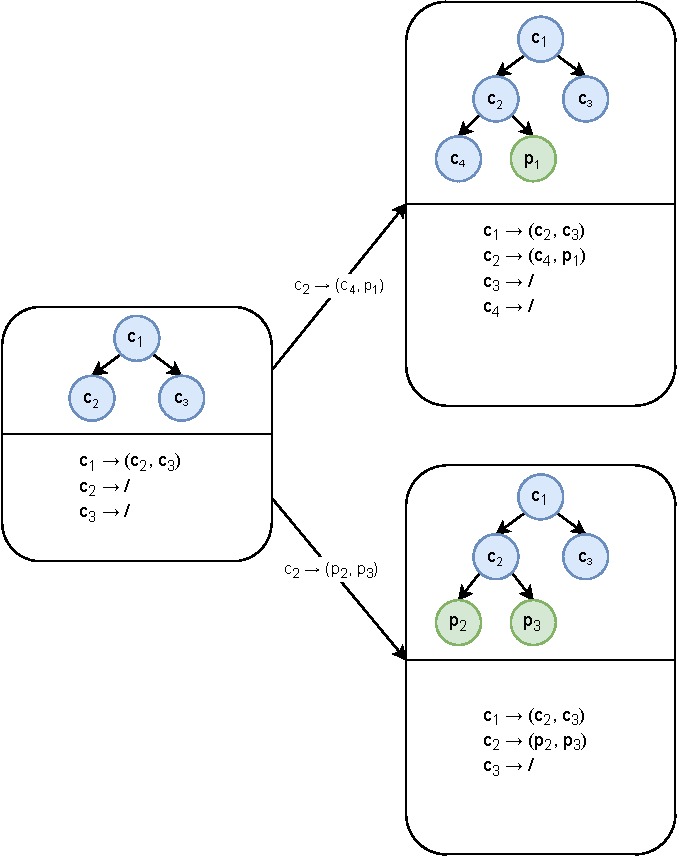
\includegraphics[height=0.5\textheight]{gfx/Figures/Approach/HTN.pdf}
    \caption{An example of a partial HTN planning search tree for a simple planning problem.
    Each node is illustrated with the task-tree for the partially solved plan up to this point in its upper half, where compound task nodes are blue and primitive task nodes are green.
    In the lower half are all involved compound tasks listed in the utilized ordering.
    If any decomposition rule was already applied for a compound task, it is listed here as well.
    The first node on the left has already utilized a decomposition for compound task $c_1$ into $c_2$ and $c_3$.
    In this ordering the first undecomposed compound task is $c_2$ and since two decomposition rules $c_2 \rightarrow (c_4, p_1)$ and $c_2 \rightarrow (p_2, p_3)$ are applicable, the node of this task-tree has two outgoing edges to nodes, where the corresponding decomposition rule was applied to the represented task tree.
    After applying the second decomposition rule, $c_2$ has solely primitive tasks as sub-tasks and can therefore be marked as solved.
    In the case of the first decomposition rule, $c_4$ needs to be decomposed and solved before $c_2$ can would be solved.
    }
    \label{fig:appraoch:htn-planning}
\end{figure}

\subsection{Description of the Search Space Graph}
\label{sec:appraoch:selection:graph}
The examples of HTN tasks in~\ref{sec:appraoch:selection:search} are given as instructions in plain english but this cannot be used in a algorithm and therefore a formalization is necessary.
With a suitable formalization and corresponding data model, the HTN planning domain is adjustable and expandable for the exact use-case and for the case of the AutoML context it is possible to modify possible pipeline topologies and the set of pipeline components that are used for construction.\newline
In a manual pipeline construction it is not possible to create arbitrary pipeline graphs because components often expect a certain type of input that can only be given by certain other components as an output.
Additionally, the selection of some components implies the requirement of selecting certain other components.
For example if an ensemble method was selected as a learning model, the components that are used to be the predictors of the ensemble must be learning model components and cannot be pre-processing models.\newline
To incorporate such constraints into tasks and decomposition rules, ML-Plan utilizes a simple type system in the form of required and provided interfaces.
Each task has one or more type definitions which represents certain properties of the solution to the associated task.
For example, the primitive task of using a Decision Tree as well as the compound task of creating an ensemble learning model out of several other learning models would both offer a solution in the form of a machine learning model.
Both of them could have something like \texttt{Classifier} or \texttt{Learner} as their solution type and therewith as the types of interfaces they provide.\newline
On the other hand, are compound tasks only solvable if they get solutions of certain types as the results of the sub-tasks they are decomposed into.
For example, a Stacking classifier can only be based other classifiers, i.e. solutions with types like \texttt{Classifier}.
Thus, each compound tasks has one or more required interface, which represents this solution types the compound task will be based on.\newline
Decomposition rules are now simple matching rules, i.e. which required interfaces can be satisfied with which provided interface.
Of course it is possible that this interface types need to be identically for simplicity.
A compound task with a required interface of type $a$ can only be decomposed into another task, which has $a$ as one of its provided interface types.
With such a definitions of required and provided interface types for each task, pipeline topology specific constraints like splits into two sub-pipelines and uniting such sub-pipelines, or machine learning specific constraints like for example creating ensembles out of classifiers, are straightforward to incorporate into the planning problem without the need to write a list of decomposition rules.\newline
The overall pipeline structure, for example Pre-Processing + Learning Model or Pre-Processing + Learning Model + Post-Processing, can be encoded in the required interfaces of the goal task.
Every actual pipeline component, which shall be included for constructing pipelines, will be represented as primitive tasks.
For a better structure, they should be grouped by their provided interface types that are deduced from their properties and purposes.
Pipeline topologies, like creating parallel pre-processing sub-pipelines can be for example achieved with a Feature Union pipeline component, which has one or more types of pre-processing components as required interfaces.
Pipelines with a dynamic length can be achieved comparable to generating sequences with an unlimited length in a regular grammar, where a pipeline can either be decomposed into just a component or a component and a pipeline.
A simple HTN planning space for a very small AutoML model selection space is illustrated in~\ref{fig:appraoch:htn-automl}.
\begin{figure}[ht!]
    \centering
    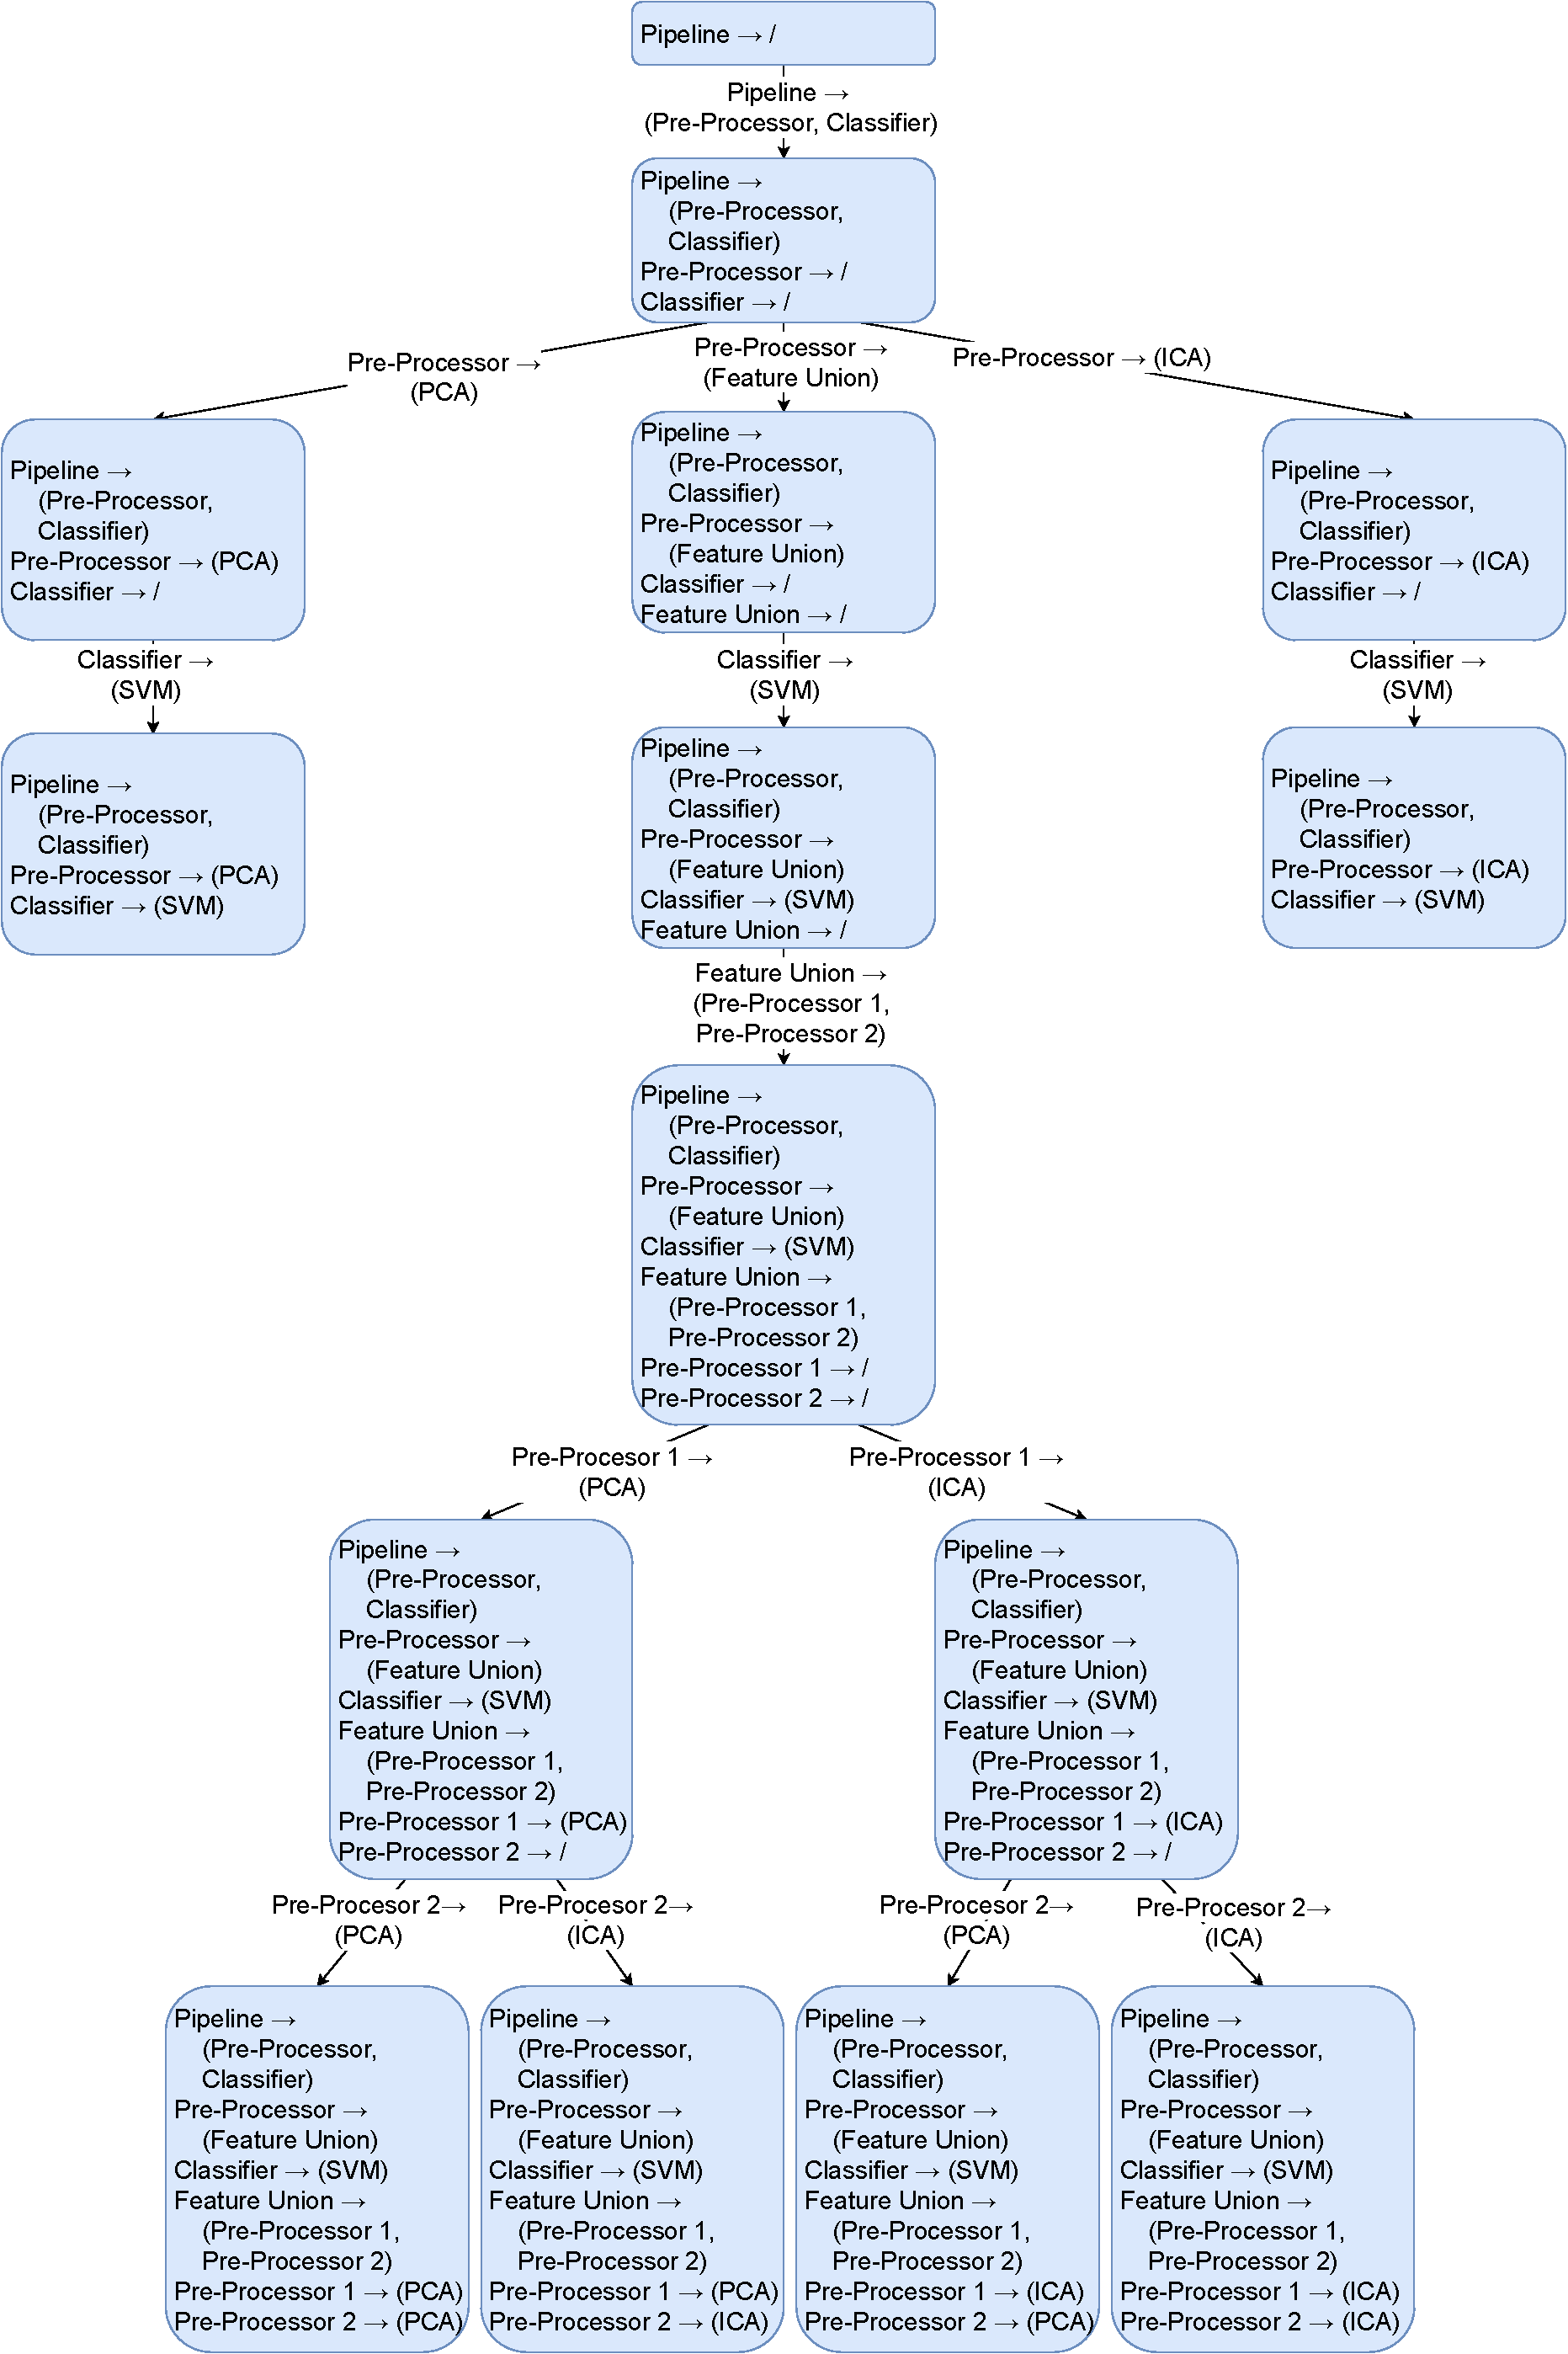
\includegraphics[width=\textwidth]{gfx/Figures/Approach/HTNAutoML.pdf}
    \caption{A complete search graph of an AutoML problem visualized in the HTN context.
    The primitive tasks are PCA, ICA, SVN and KNN.
    All available compound tasks are Pipeline, Pre-Processor, Classifier, Feature Union, First Pre-Processor and Second Pre-Processor.}
    \label{fig:appraoch:htn-automl}
\end{figure}

\subsection{Multiple Optimization Algorithms as a Multi-Armed Bandit Problem}
\label{sec:appraoch:selection:bandit}
When all compound tasks are solved and therefore a leaf node $n^*$ of the search space is reached, all components of the pipeline are selected and for this node with its pipeline it can be deduced which parameters each component needs a configuration space and therefore which is the model configuration space.
To enable an actual model configuration with one of the available optimization algorithms, or theoretically even different configurations of the same algorithms, $A = \{ a_1, ..., a_k \}$, one additional node for each $a_i \in A$ will be attached as a child of $n^*$.
Therefore, the search tree $G=(V, E)$ of the HTN planning is extended for $A$ in the form of $V'=V \cup \{n^*_{a_1}, ..., n^*_{a_k}\}$, $E'=E \cup \{(n^*, n^*_{a_1}), ..., (n^*, n^*_{a_k})\}$, $G' = (V', E')$.
An simplified illustration without the HTN planning aspects of this extended search tree can be seen in figure~\ref{fig:appraoch:search-graph}.
\begin{figure}[ht!]
    \centering
    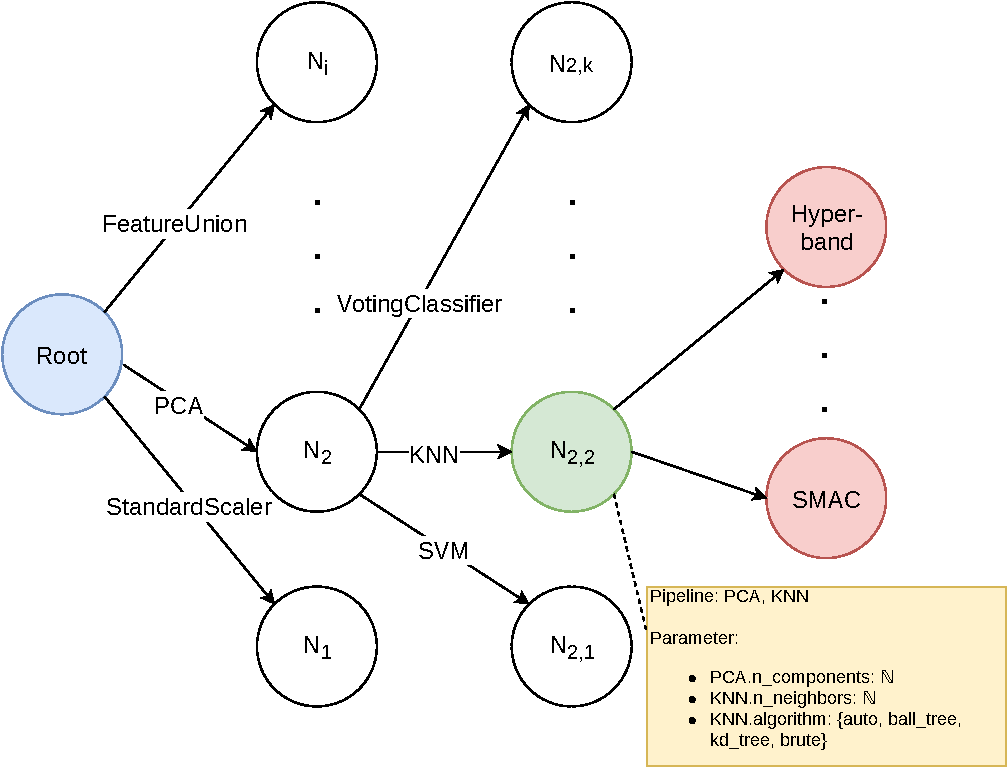
\includegraphics[width=\textwidth]{gfx/Figures/Approach/SearchGraph.pdf}
    \caption{A simplified illustration of the search tree. The root is drawn in blue, the inner nodes in white, a node with a fully constructed pipeline in green and the additional nodes for optimizing the parametrization of this pipeline in red.
    The yellow box shows the configuration space of the pipeline.}
    \label{fig:appraoch:search-graph}
\end{figure}
Now, the challenge arises to select one of the optimization algorithms for the model configuration step of a pipeline $p$.
But there exists no prior knowledge, which optimizer is the most suitable one for this configuration space.
It is possible that for example $a_1$ is the best algorithm for optimizing the parametrization of this concrete $p$.
Alternatively it could also be the case for this example that algorithm $a_2$ is the best choice for generally optimizing all possible configurations spaces of pipelines that contain an ICA component and therefore is the best optimizer choice for the complete sub-tree below the selection of the ICA component which could include this pipeline $p$ as well.\newline
Until such knowledge is collected, there is no other choice but to try out different optimization algorithms for optimizing the parametrization of $p$ and examine their optimization results.
This try-and-error approach is also referred to as \textit{exploration}.
During the collection of exploration results it will become more evident, which optimizer yields which score quality.
But this score observations of one optimizer are equatable to an experiment that has an underlying random variable with an unknown distribution.
Without a high number of observations it is not possible to factually assess an optimizers score quality for $p$ without uncertainty.
Thus, the currently best scored algorithm could be not the overall best one and with further exploration of other optimizers the true best one could be found.
But because there is a limited optimization budget, it is not a productive approach to solely explore the different candidates.
From time to time the best optimizer explored up to that point should be utilized since it can perform the most promising optimization to the best of the collected knowledge.
This utilization of the candidate with the best observed scores is also referred to as \textit{exploitation}.
A balanced strategy between exploration and exploitation is the core concept of \textit{Multi-Armed Bandit} problems, which are the theoretical foundation of the model selection method and the selection of an model configuration optimizer in this appraoch.

\subsection{Ensemble Interaction with a MCTS}
\label{sec:appraoch:selection:mcts}

\Blindtext

\section{Model Configuration with Multiple Optimizers}
\label{sec:approach:configuration}

\Blindtext

\subsection{Shared Parameter Domain for Selected Models}
\label{sec:appraoch:configuration:parameter}

\Blindtext

\subsection{Warmstarting Versions of Optimization Algorithms}
\label{sec:appraoch:configuration:warmstart}

\Blindtext